   \chapter{Upper Limb Exoskeleton With One Degree of Freedom}
   
   \label{ch:ulexo}
   
   This chapter briefly describes an upper limb exoskeleton with one degree of freedom already available at the Biomechatronics laboratory. A more extensive description of this system can be found at \cite{Sommer2015}.
   
   \section{Mechanical}
   
   \subsection{Structure}
   
   The exoskeleton structure is made of aluminum bars. The aluminum structure is attached to a Power Window Lifter steel mechanism.
   
   The user's arm is placed at the aluminum structure and held firmly through the use of rubber straps.
   
   \begin{figure}[thpb]
      \centering
      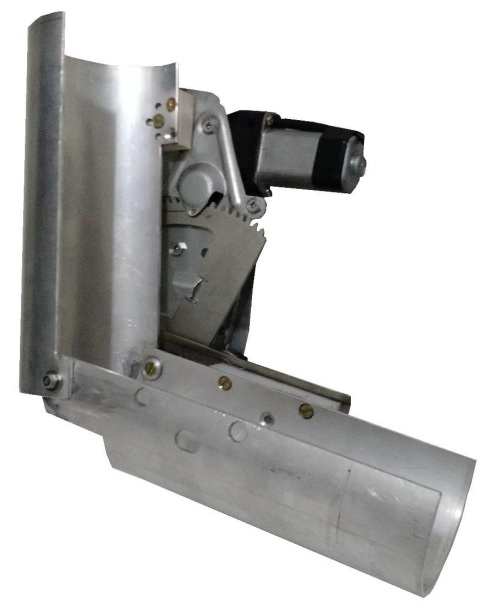
\includegraphics[scale=0.5]{Images/Exoskeleton.jpg}
      \caption{Upper limb exoskeleton with one degree of freedom \cite{Sommer2015}}
      \label{exoskeleton}
   \end{figure}
   
   \subsection{Actuator}
   
   The actuator of the exoskeleton is composed by a Mabuchi JC-578VA-4720 DC motor and a Power Window Lifter mechanism.
   
   This DC Motor was chosen because of its high power-to-weight ratio, low dimensions and low price.
   
   In order to increase the motor torque, the DC motor is attached to a modified Power Window Lifter, a mechanism with gear coupling with a reduction factor of 10:1.
   
   \begin{figure}[thpb]
      \centering
      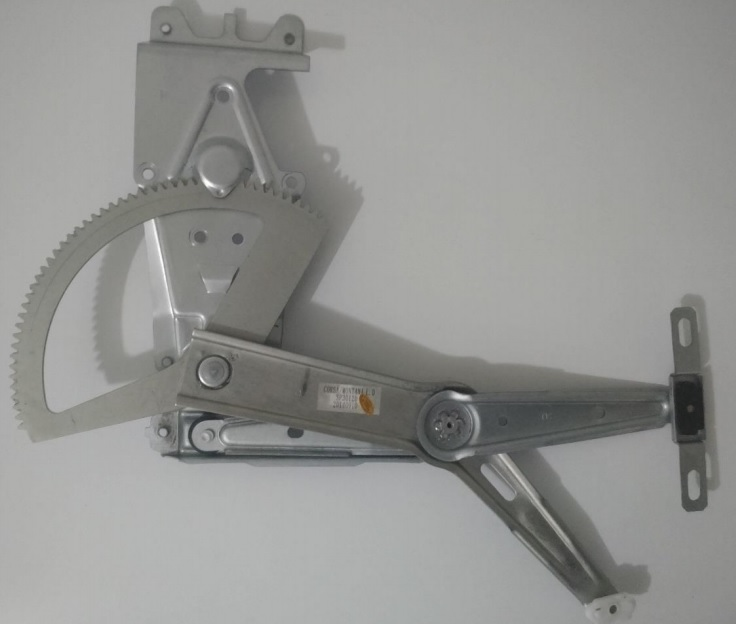
\includegraphics[scale=0.5]{Images/PowerWindowLifter.jpg}
      \caption{Power Window Lifter \cite{Sommer2015}}
      \label{PowerWindowLifter}
   \end{figure}
   
   \section{Electronics}
   
   The electronics system of the exoskeleton is composed of the following parts: An sEMG sensor, that acquires the sEMG signal of the target muscle; a microprocessor to process the analog sEMG signal, apply the control logic and output a PWM signal; a motor driver that receives the PWM signal as input and outputs the necessary power to drive the DC motor.
   
   \begin{figure}[thpb]
      \centering
      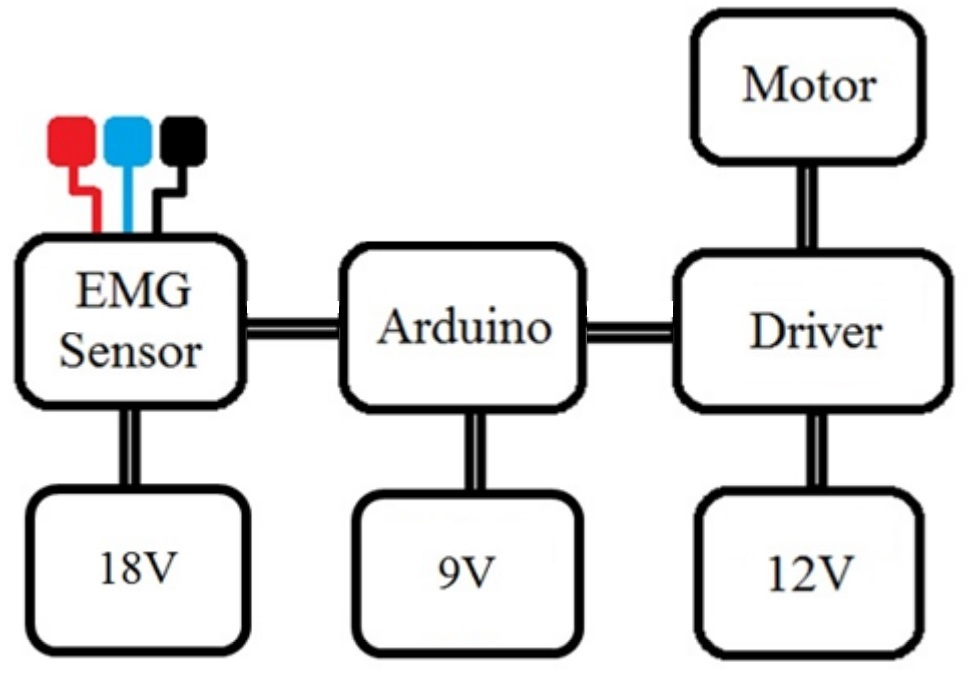
\includegraphics[scale=0.5]{Images/ElectronicSchematic.jpg}
      \caption{Schematic of the electronics \cite{Sommer2015}}
      \label{ElectronicSchematic}
   \end{figure}
   
   \subsection{EMG Sensor}
   
   The EMG Sensor is a SparkFun Muscle Sensor V3. 
   
   Three electrodes are attached to this sensor: Two electrodes are placed at the target muscle and measure the difference of electrical activity and one is placed at an electrically neutral region of the body, like a bony area, and serves as the ground signal.
   
   The signal from the electrodes is differentially amplified in the AD8221 amplifier; then, the signal is amplified twice by TL084 operational amplifiers; the signal is rectified using 1N4148 diodes; the rectified signal is attenuated by a filter; at last, the signal is amplified with an adjustable gain.
   
   The Sensor output is sent directly to the microprocessor. 
   
%    \begin{figure}[thpb]
%       \centering
%       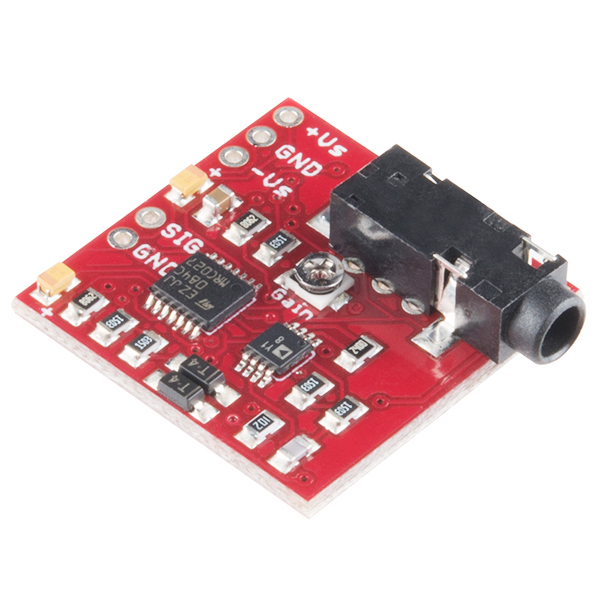
\includegraphics[height=0.3\textheight]{Images/MuscleSensorV3.jpg}
%       \caption{Muscle Sensor V3 \cite{musclesensorv3}}
%       \label{MuscleSensorV3}
%    \end{figure}
   
   \subsection{Microprocessor}
   
   The microprocessor is an Arduino UNO. It was chosen for its low cost, ease-of-use, extensive available documentation and easy communication to the Muscle Sensor V3. It has a built-in Analog/Digital converter and is capable of emitting PWM signals. Also, it is possible to connect more sensors to this microprocessor, for future adaptations of the exoskeleton.  

   
   \subsection{Driver}
   
   The DC motor demands electrical currents up to 24A. Motor Drivers for 12V, 24A DC motors are expensive. For this reason, a motor driver was designed for the specific use on this exoskeleton.
   
   The driver has two inputs (clockwise rotation and counter-clockwise rotation) that receives the PWM signal from the microprocessor for the desired direction of motion. There are two outputs that are connected to each one of the motor electrical terminals.
   
%    \begin{figure}[thpb]
%       \centering
%       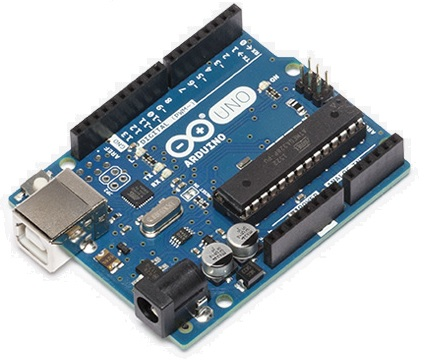
\includegraphics[height=0.3\textheight]{Images/arduino.jpg}
%       \caption{Arduino UNO. Image adapted from \cite{arduino}}
%       \label{arduino}
%    \end{figure}
   
   The driver is composed of a H-Bridge of MOSFETs. The chosen components were IRF4905 for P channel and IRLB3813 for N channel. The gate of the P channel MOSFET is powered by a TIP122 transistor.
   
   To avoid the situation where every MOSFET of the H-Bridge is activated at the same time, which would cause a short circuit between the poles of the battery, a protection circuit was implemented. The protection circuit is composed of 74LS08 AND gates and 74LS04 NOT gates. In case both the inputs are powered, no signal reaches the gates of transistors, protecting the circuit.
   
      